\section{Sea Ice Now Forecasting} %4.2

\subsection{Linear Regression} %4.2.1


\begin{figure}[htbp]
\centering
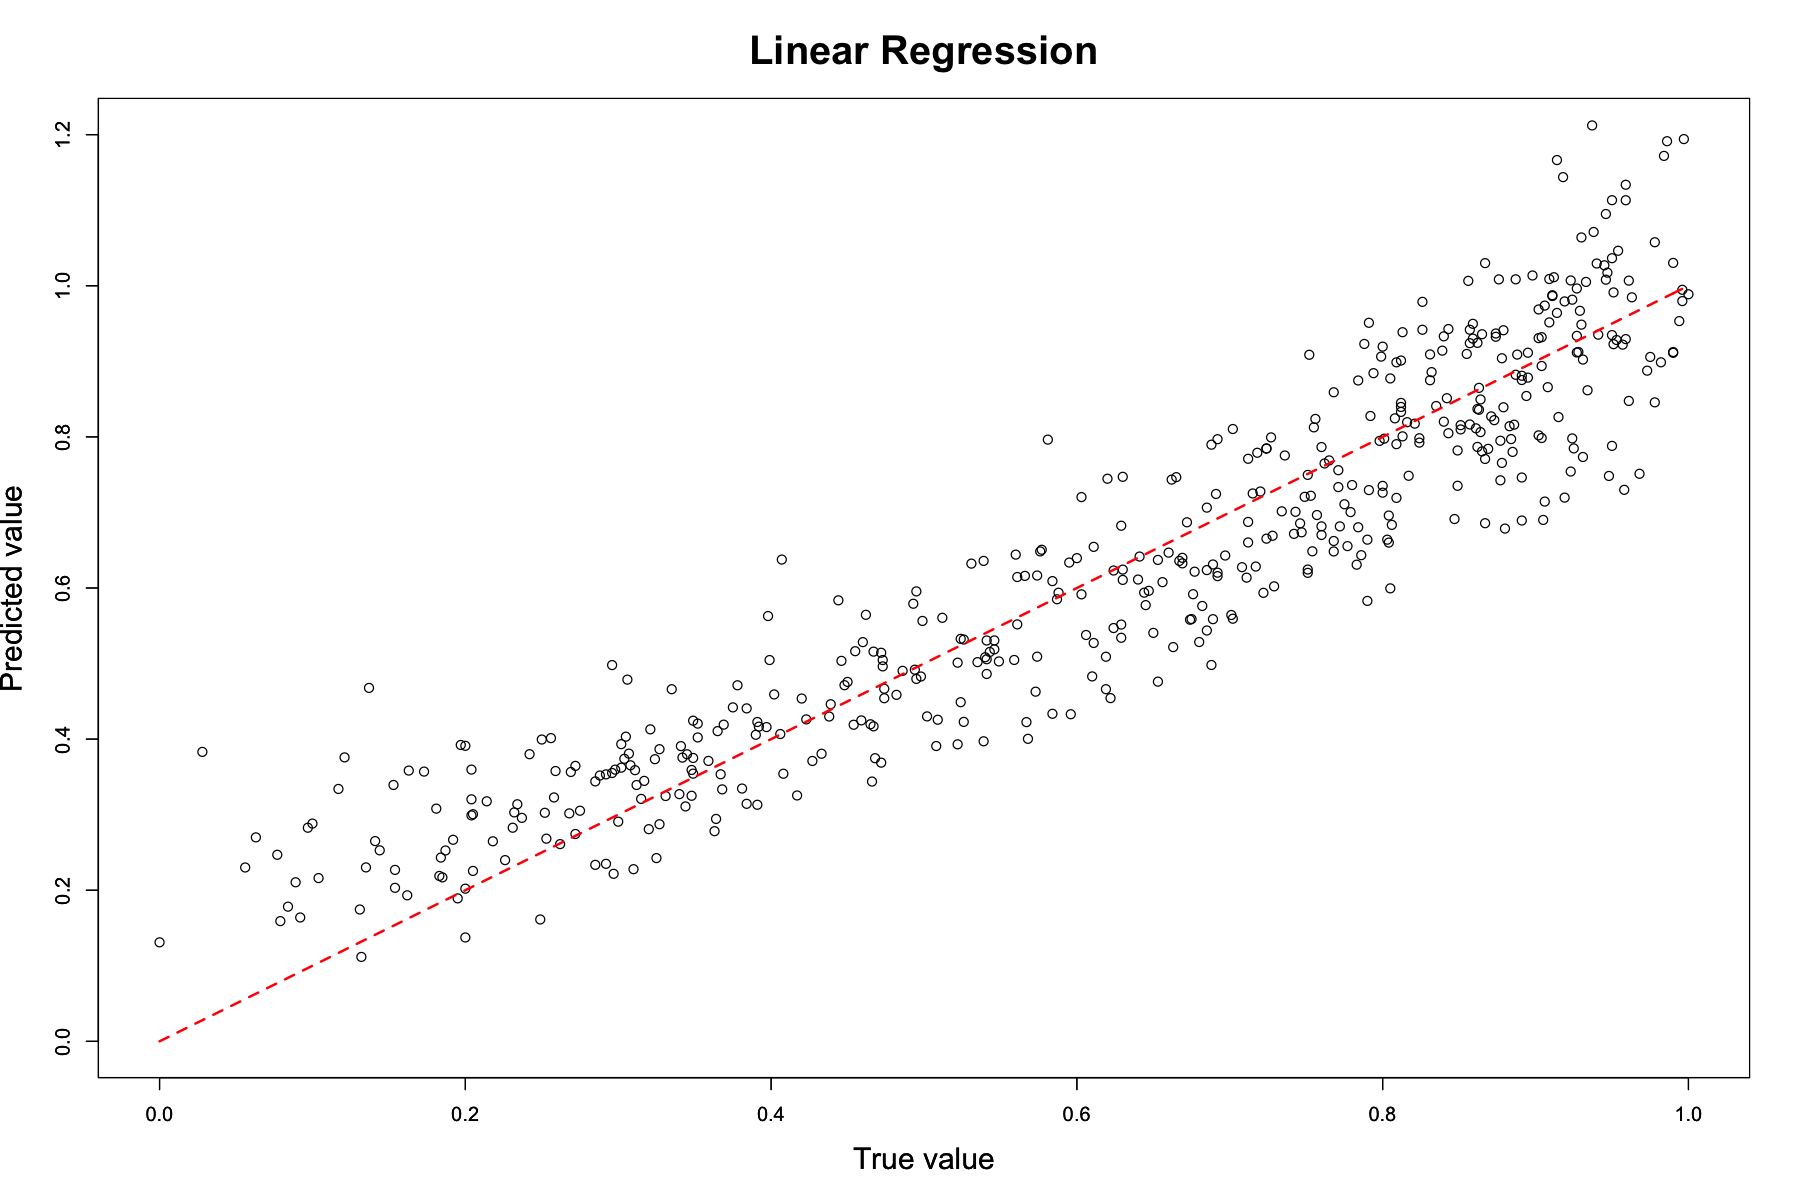
\includegraphics[width = 1.0\textwidth]{Figure/4.2.1-LR.png}
\caption{The predicted Arctic sea ice extent value vs the real Arctic sea ice extent value with k-fold Linear Regression. The red referenced dotted line represents the straight line y=x. Mean Square Error (MSE) is 0.00946.}
\label{4.2.1-LR}
\end{figure}



\subsection{Penalised Linear Regression (Lasso, min)} %4.2.2

\begin{figure}[htbp]
\centering
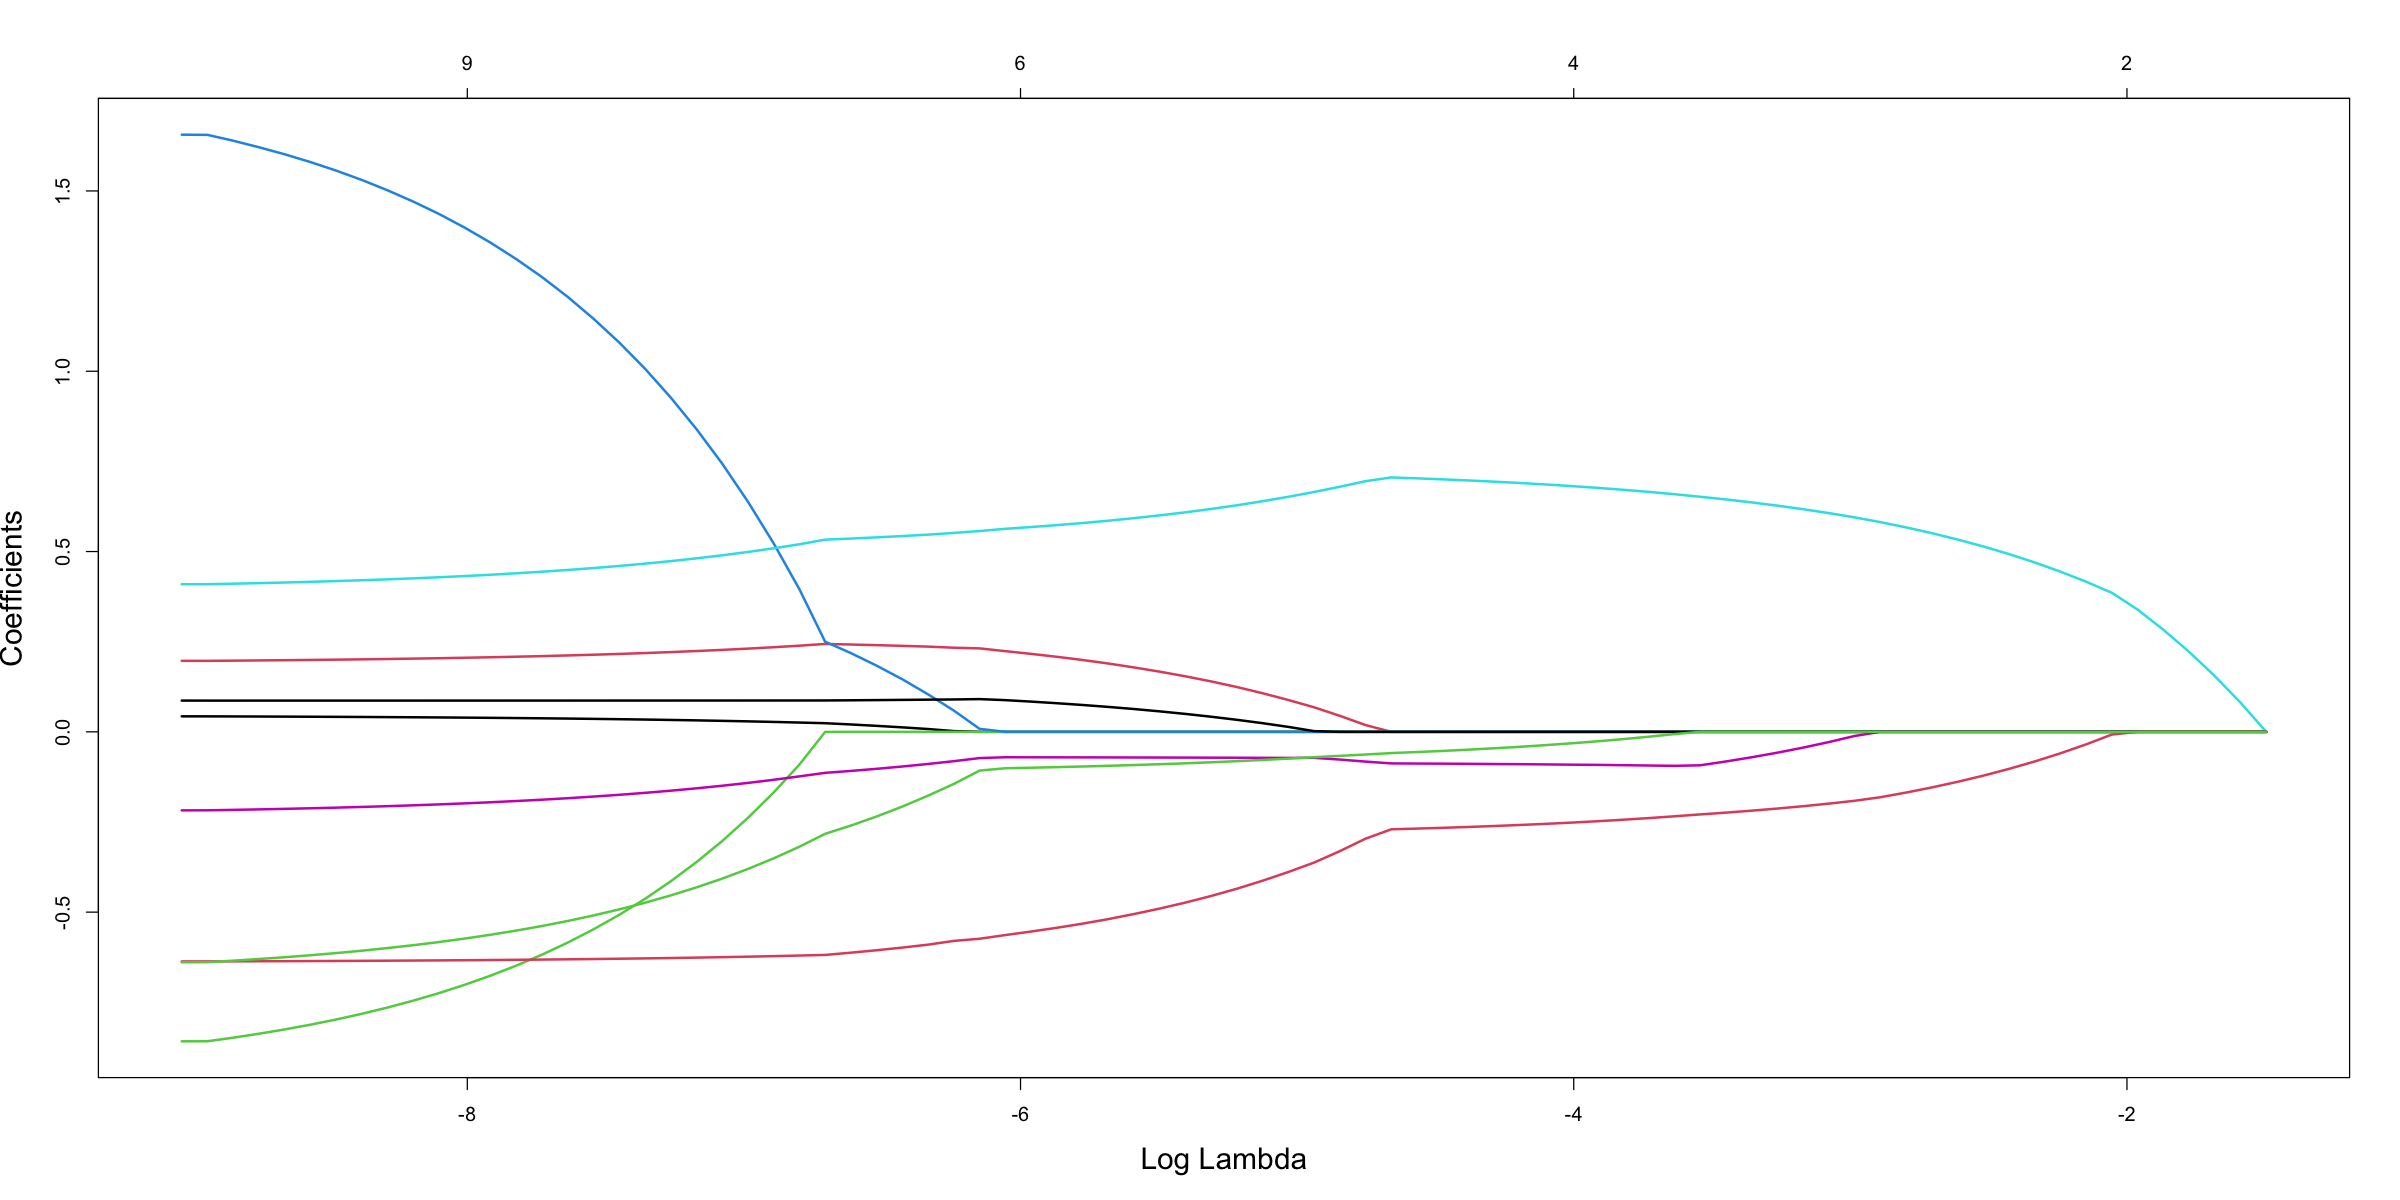
\includegraphics[width = 1.0\textwidth]{Figure/4.2.2-PLR-ridge-trance.png}
\caption{Ridge trace diagram of Penalised Linear Regression}
\label{4.2.2-PLR-ridge-trance}
\end{figure}

\begin{figure}[htbp]
\centering
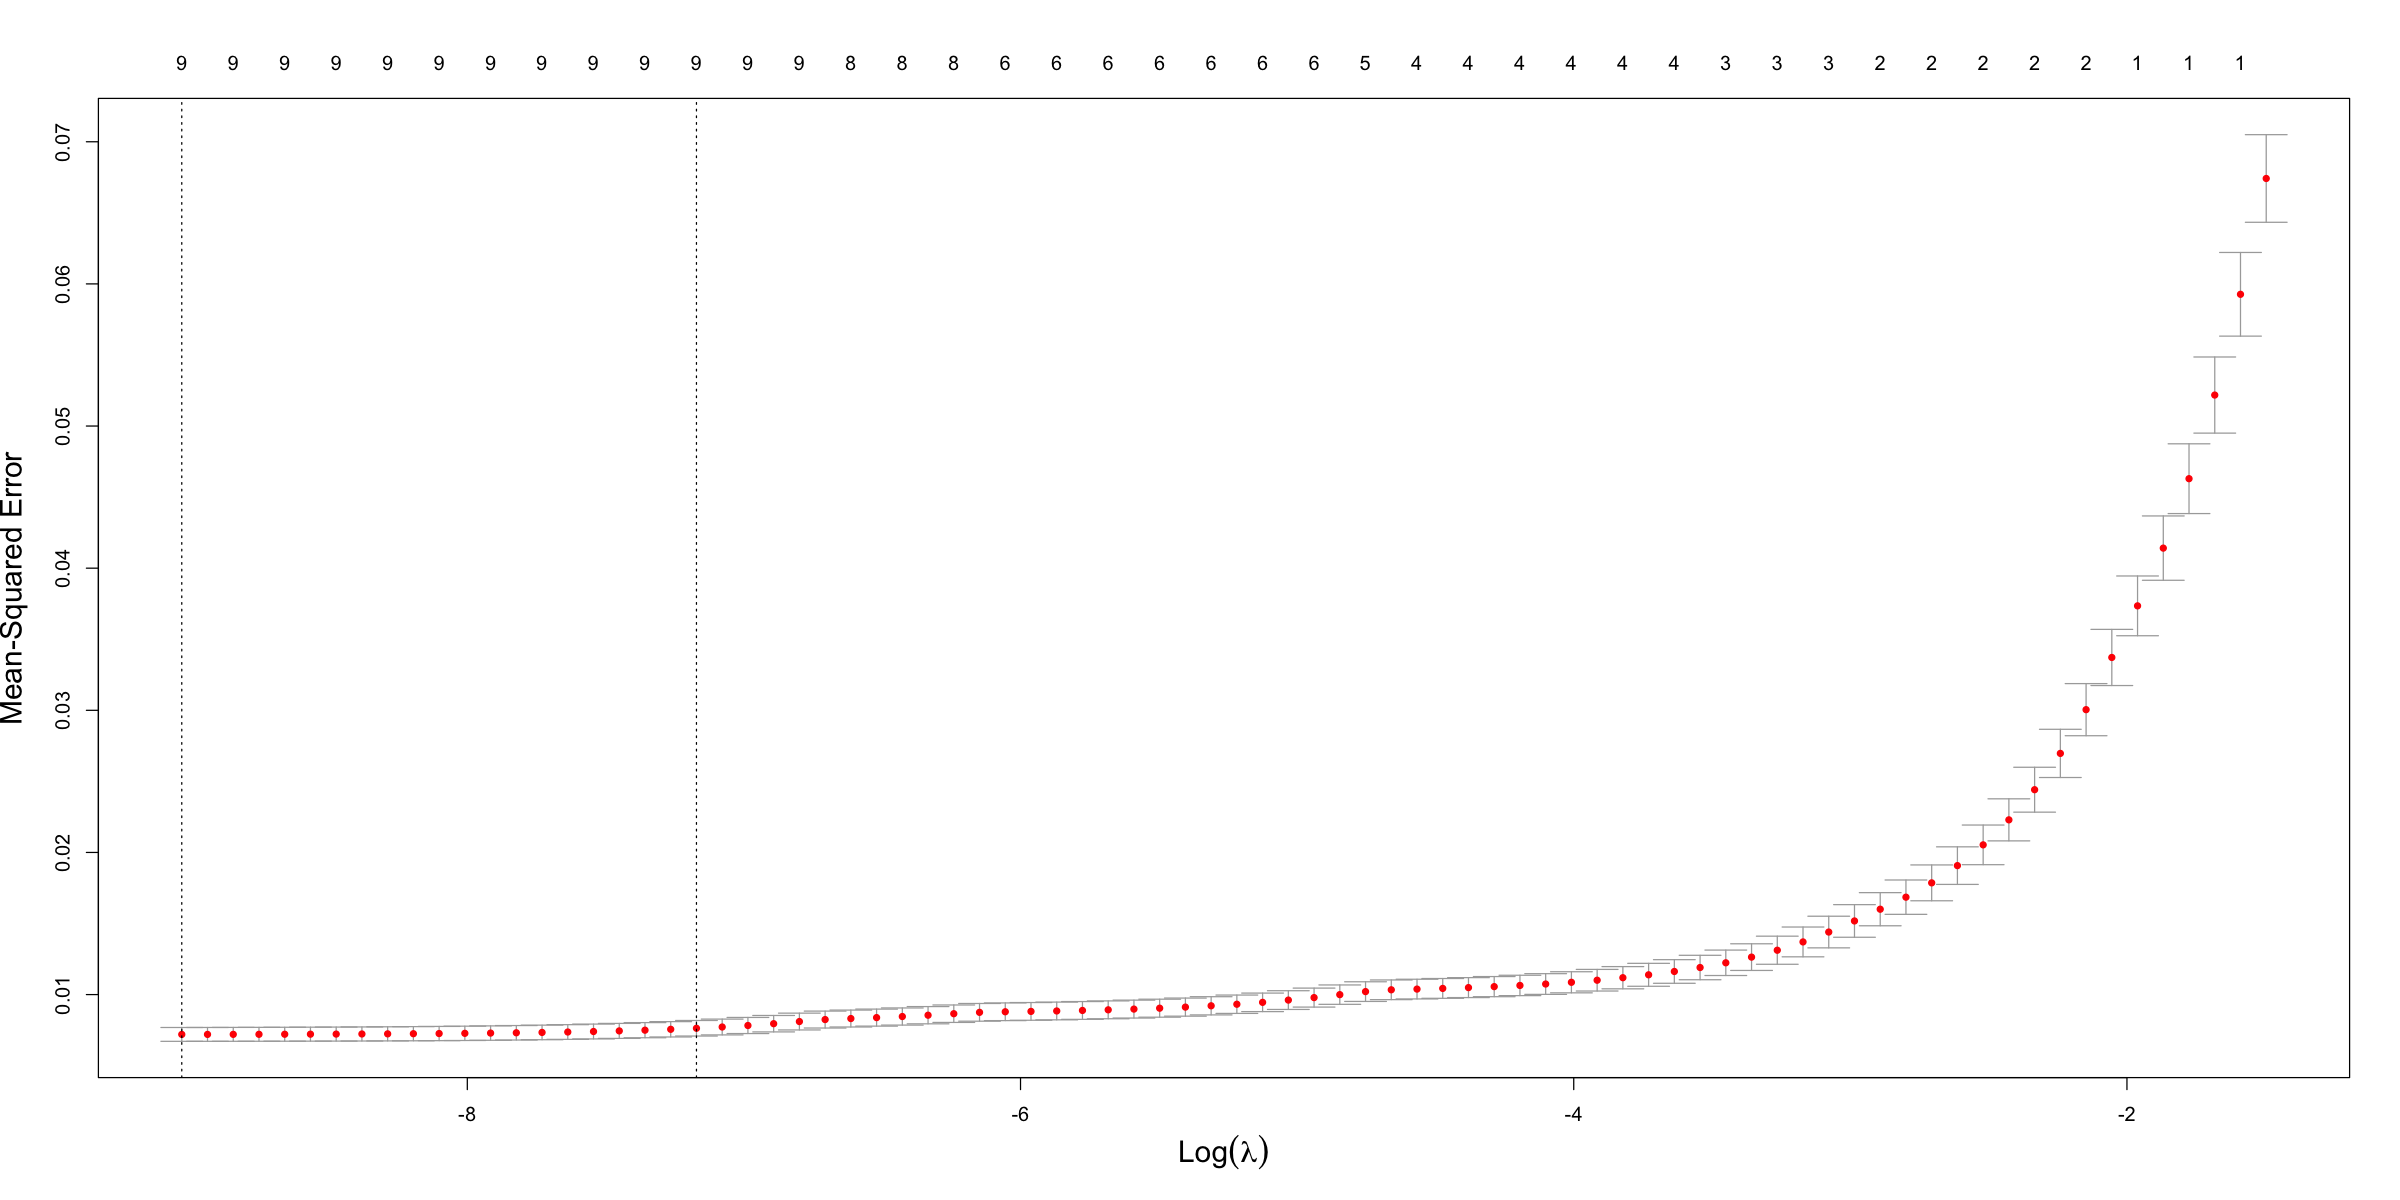
\includegraphics[width = 1.0\textwidth]{Figure/4.2.2-PLR-Log-Lambda-vs-Testing-Error.png}
\caption{Log Lambda vs Testing Error diagram of Penalised Linear Regression}
\label{4.2.2-PLR-Log-Lambda-vs-Testing-Error}
\end{figure}


\begin{figure}[htbp]
\centering
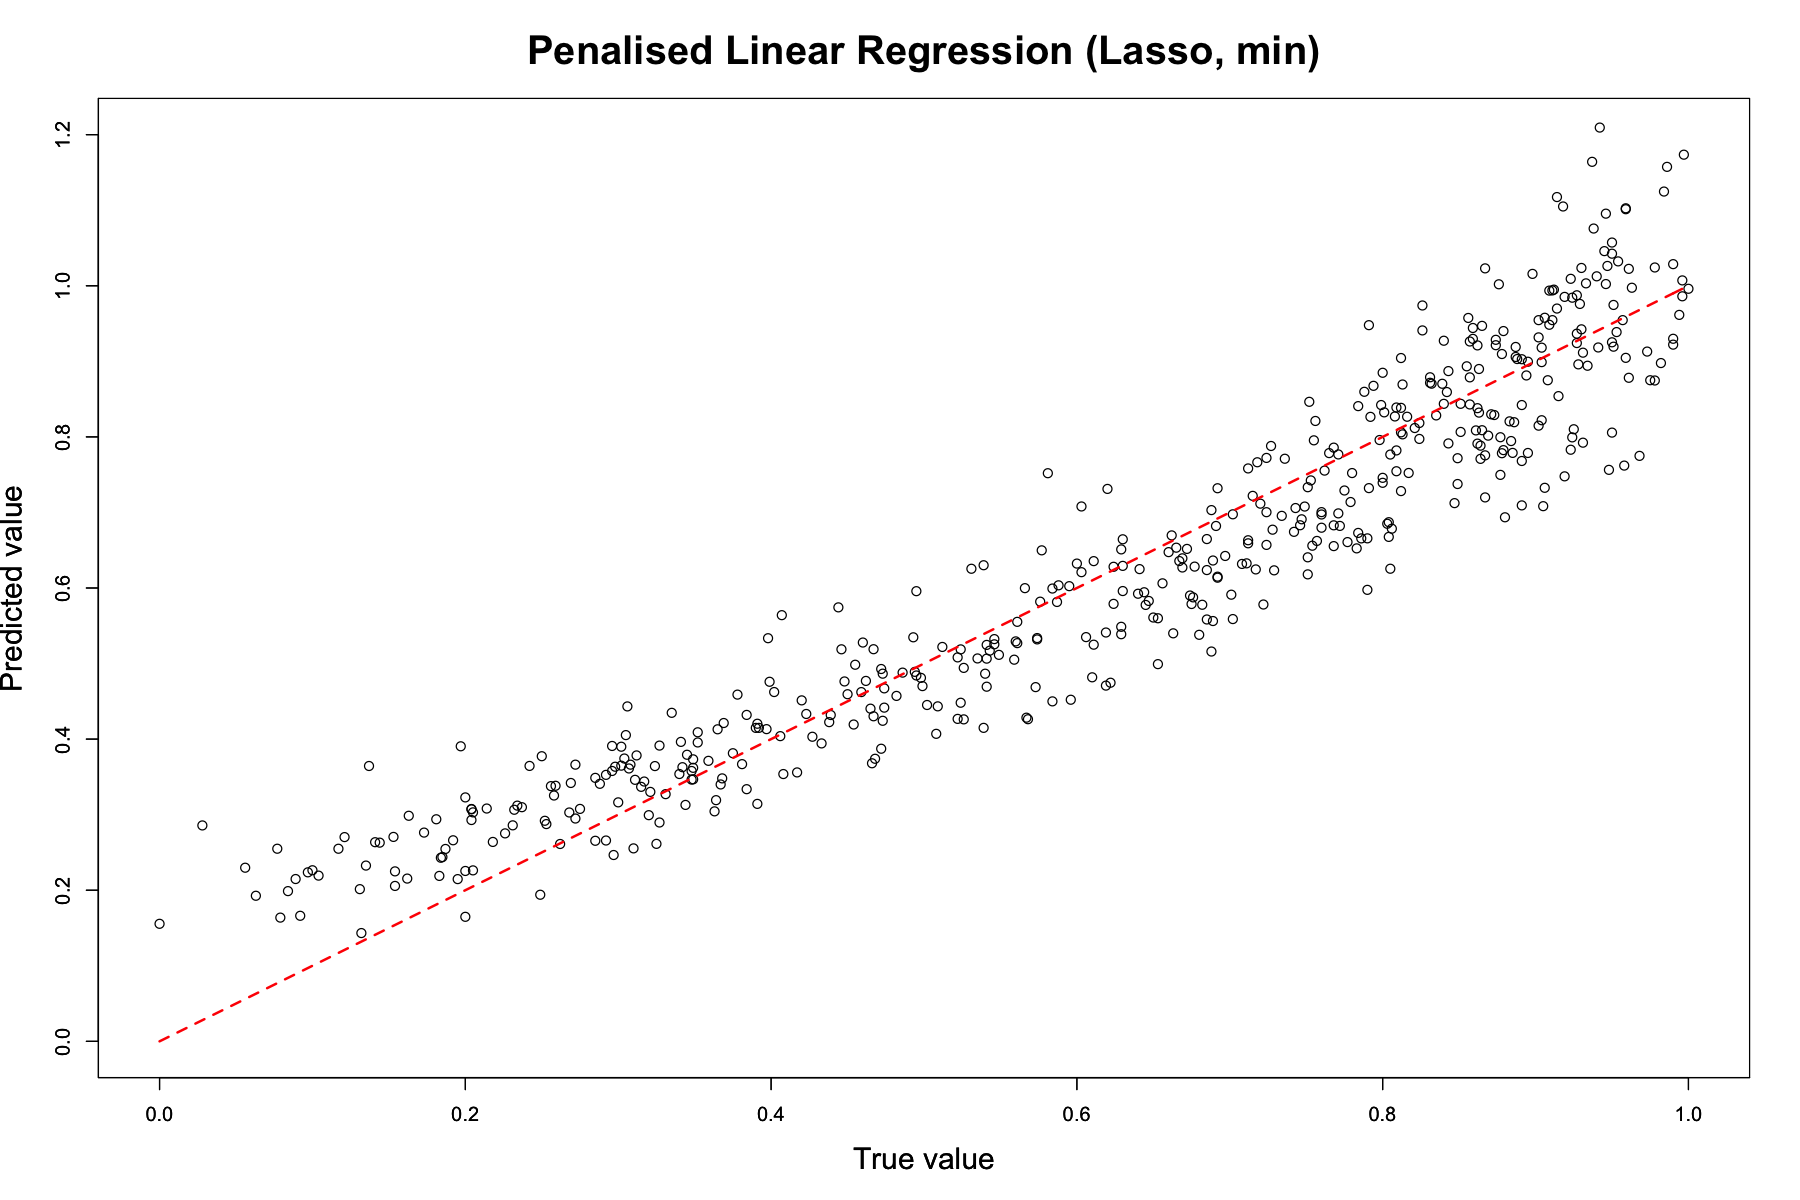
\includegraphics[width = 1.0\textwidth]{Figure/4.2.2-PLR-min.png}
\caption{The predicted Arctic sea ice extent value vs the real Arctic sea ice extent value with Penalised Linear Regression (Lasso, min). The red referenced dotted line represents the straight line y=x. Mean Square Error (MSE) is 0.00690.}
\label{4.2.2-PLR-min}
\end{figure}



\subsection{Penalised Linear Regression (Lasso, 1se)} %4.2.3

\begin{figure}[htbp]
\centering
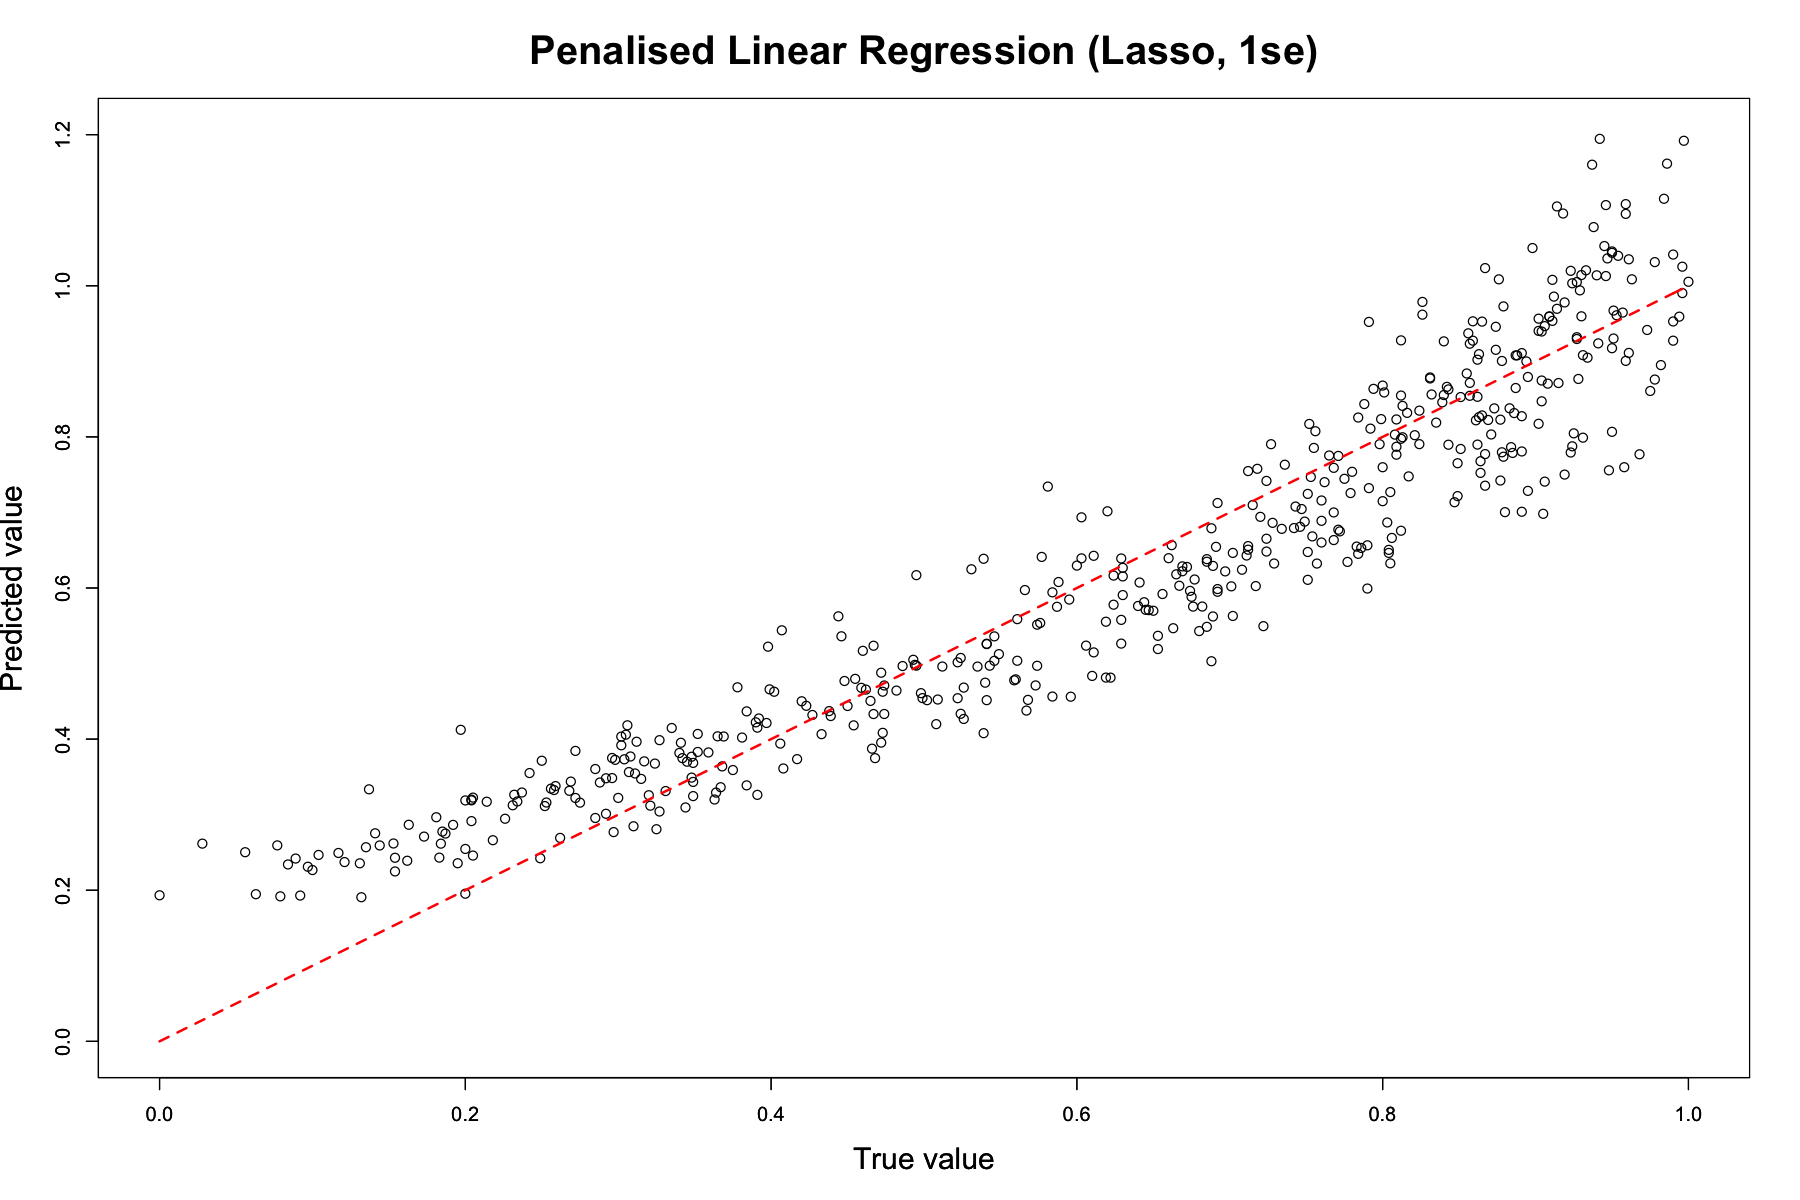
\includegraphics[width = 1.0\textwidth]{Figure/4.2.3-PLR-1se.png}
\caption{The predicted Arctic sea ice extent value vs the real Arctic sea ice extent value with Penalised Linear Regression (Lasso, 1se). The red referenced dotted line represents the straight line y=x. Mean Square Error (MSE) is 0.00732.}
\label{4.2.3-PLR-1se}
\end{figure}



\subsection{Penalised Polynomial Regression (Lasso, min)} %4.2.4

\begin{figure}[htbp]
\centering
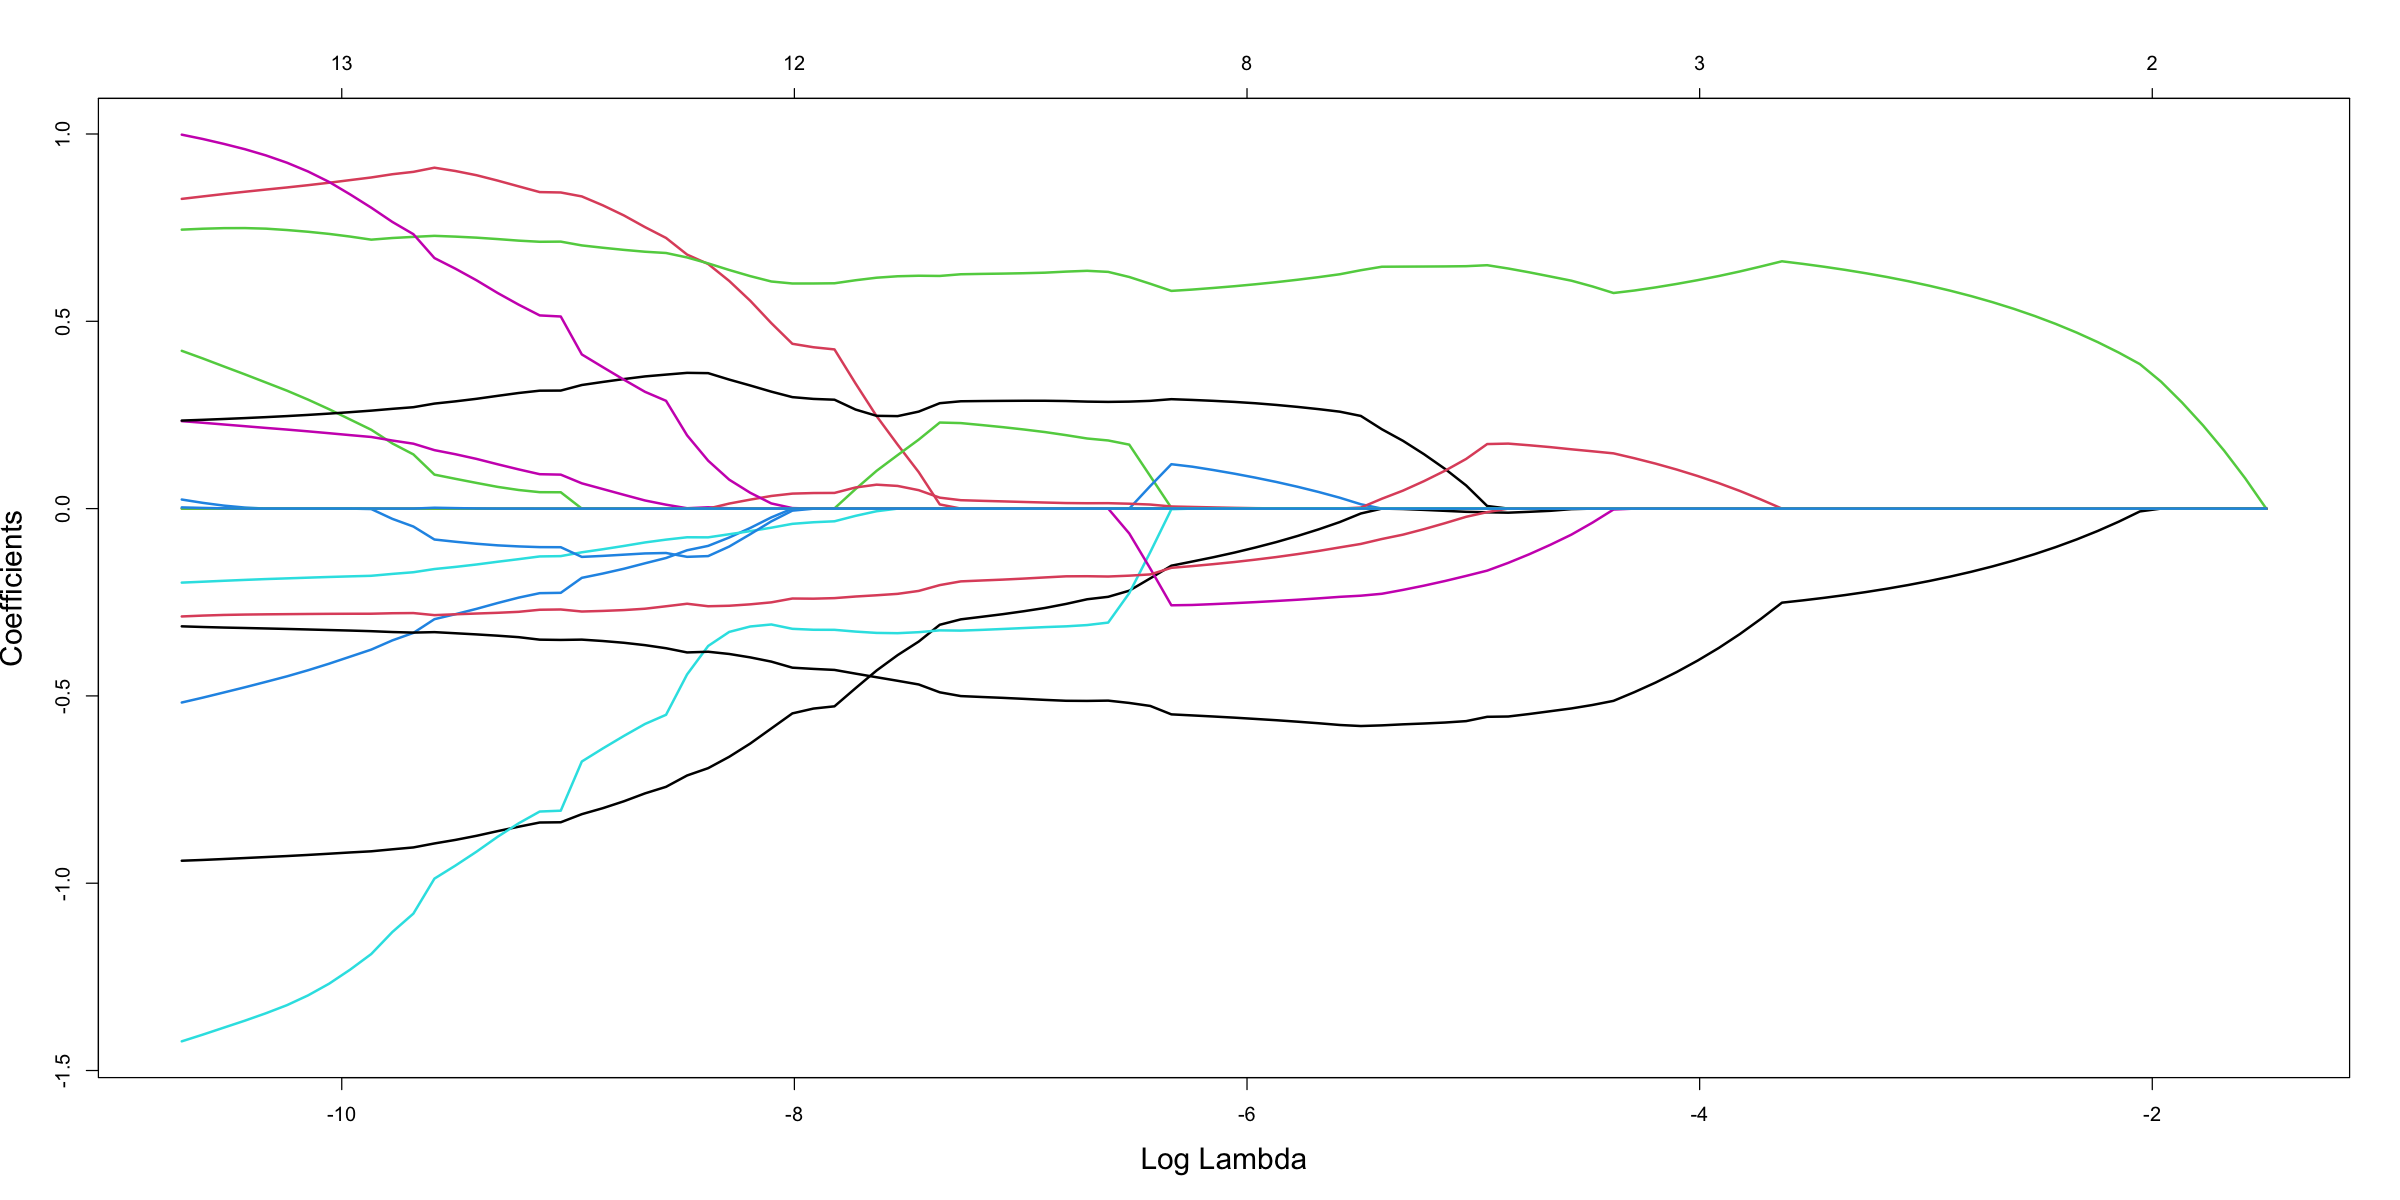
\includegraphics[width = 1.0\textwidth]{Figure/4.2.4-PPR-ridge-trance.png}
\caption{Ridge trace diagram of Penalised Polynomial Regression}
\label{4.2.4-PPR-ridge-trance}
\end{figure}

\begin{figure}[htbp]
\centering
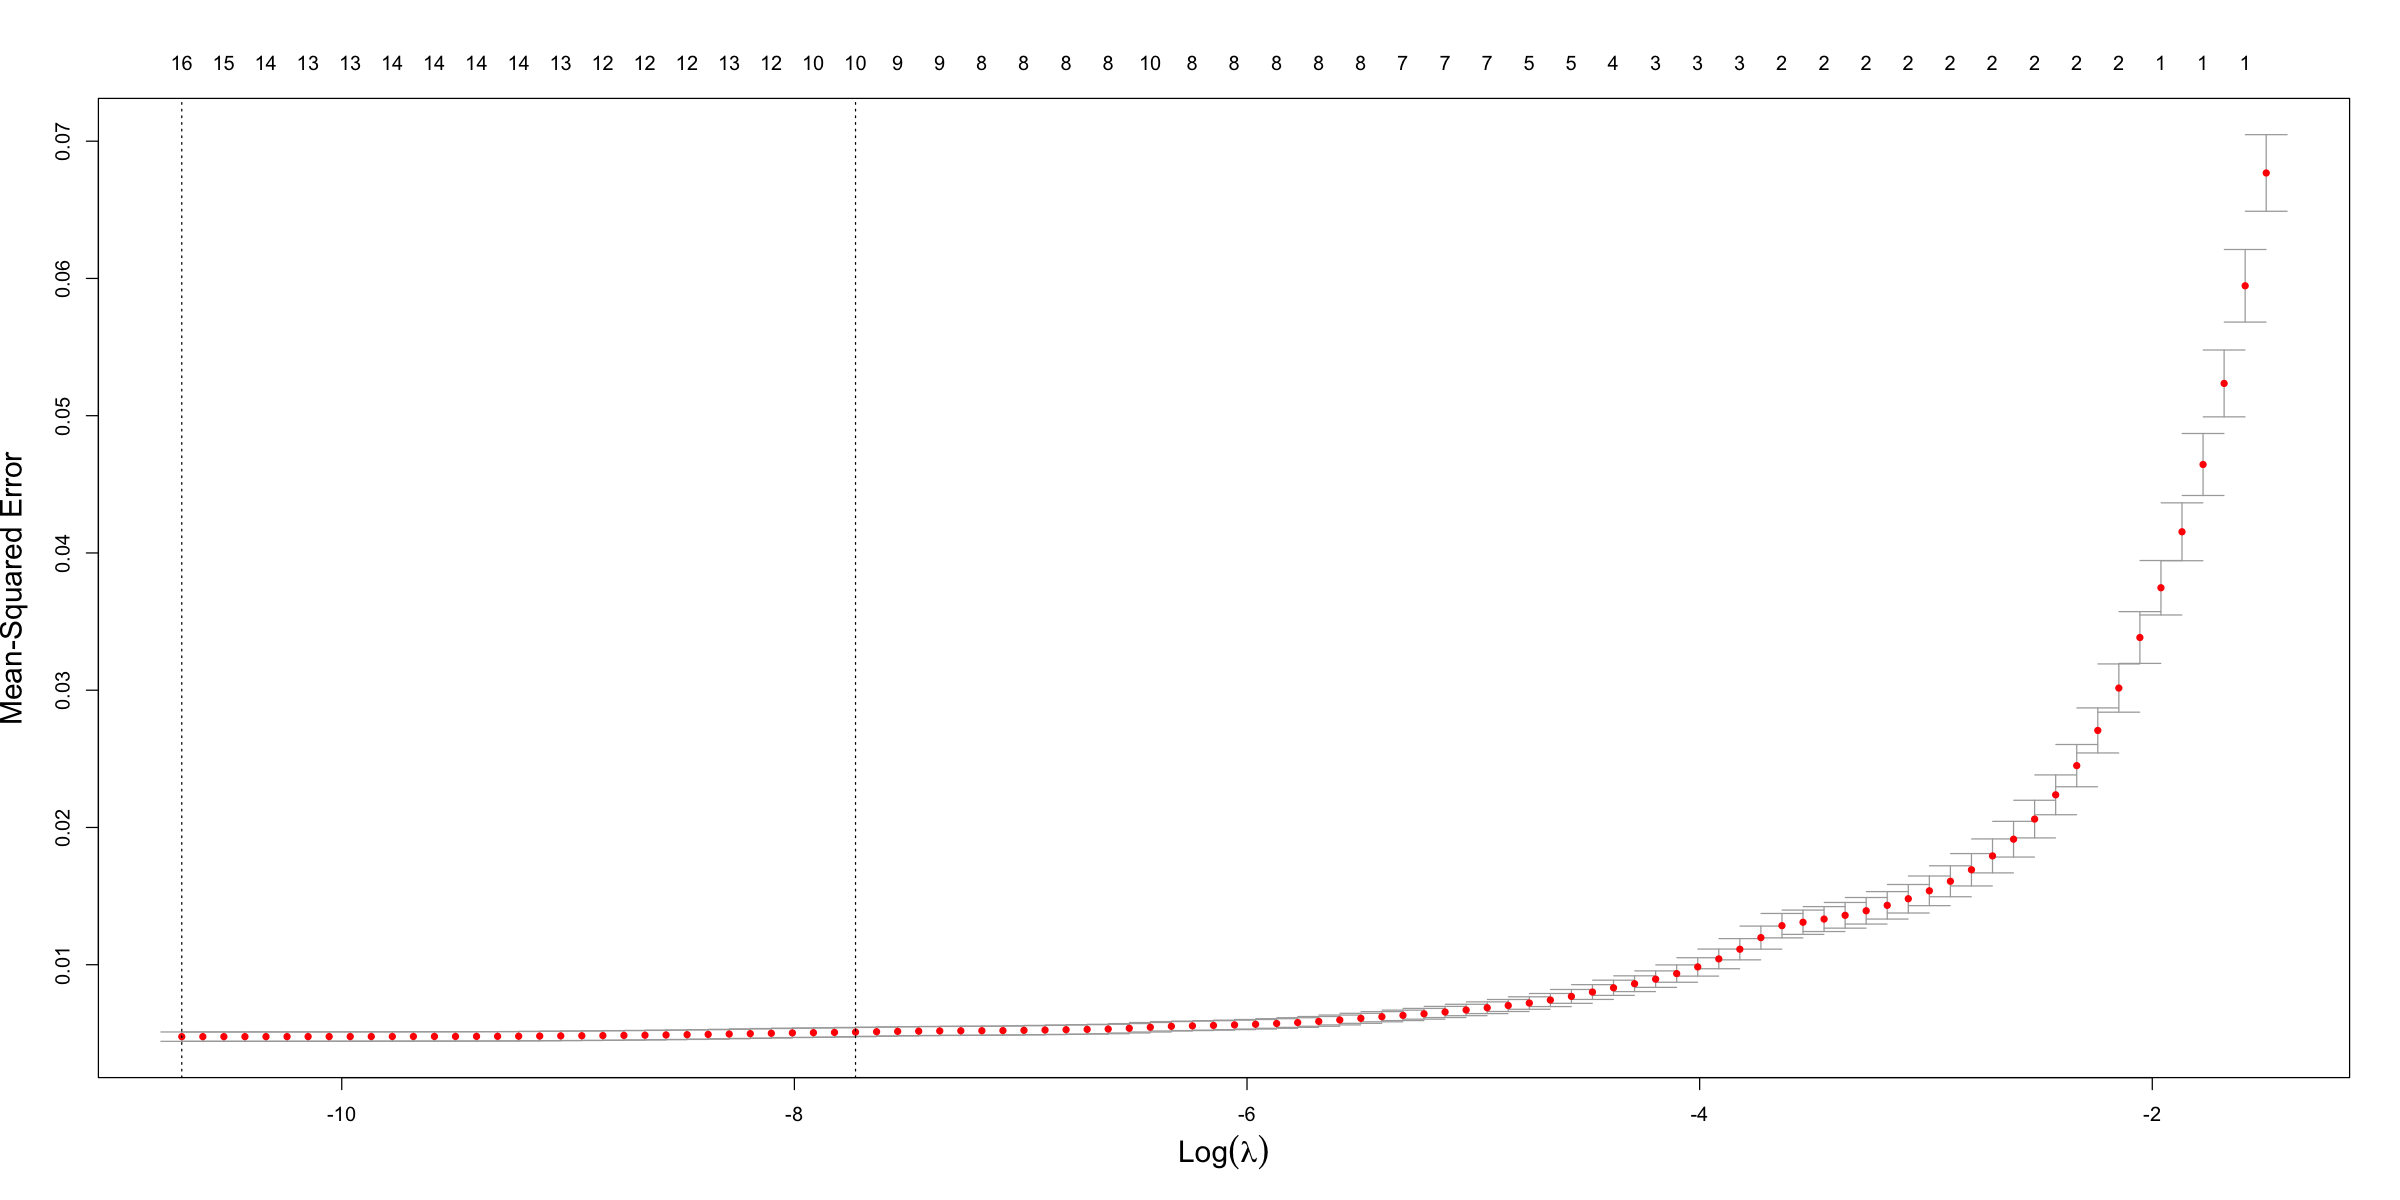
\includegraphics[width = 1.0\textwidth]{Figure/4.2.4-PPR-Log-Lambda-vs-Testing-Error.png}
\caption{Log Lambda vs Testing Error diagram of Penalised Polynomial Regression}
\label{4.2.4-PPR-Log-Lambda-vs-Testing-Error}
\end{figure}

\begin{figure}[htbp]
\centering
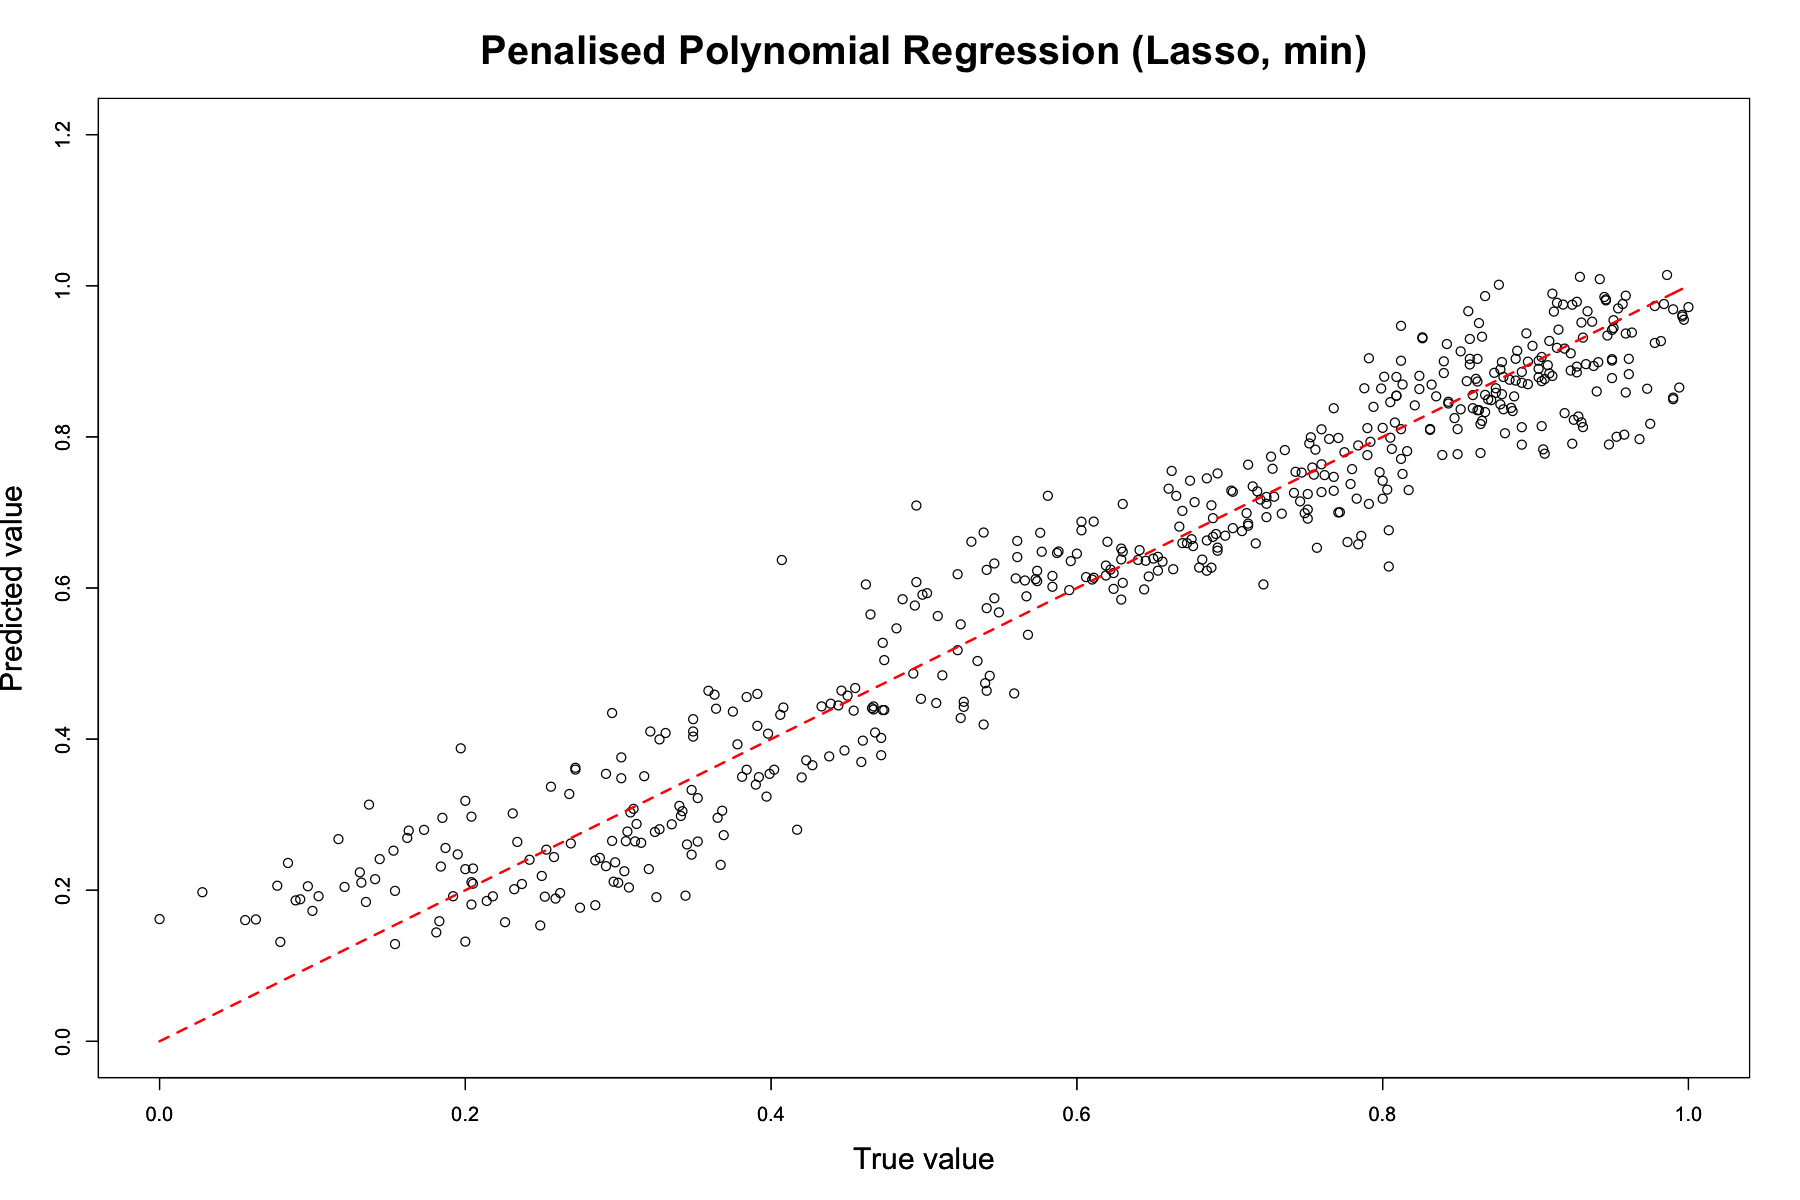
\includegraphics[width = 1.0\textwidth]{Figure/4.2.4-PPR-min.png}
\caption{The predicted Arctic sea ice extent value vs the real Arctic sea ice extent value with Penalised Polynomial Regression (Lasso, min). The red referenced dotted line represents the straight line y=x. Mean Square Error (MSE) is 0.00448.}
\label{4.2.4-PPR-min}
\end{figure}



\subsection{Penalised Polynomial Regression (Lasso, 1se)} %4.2.5

\begin{figure}[htbp]
\centering
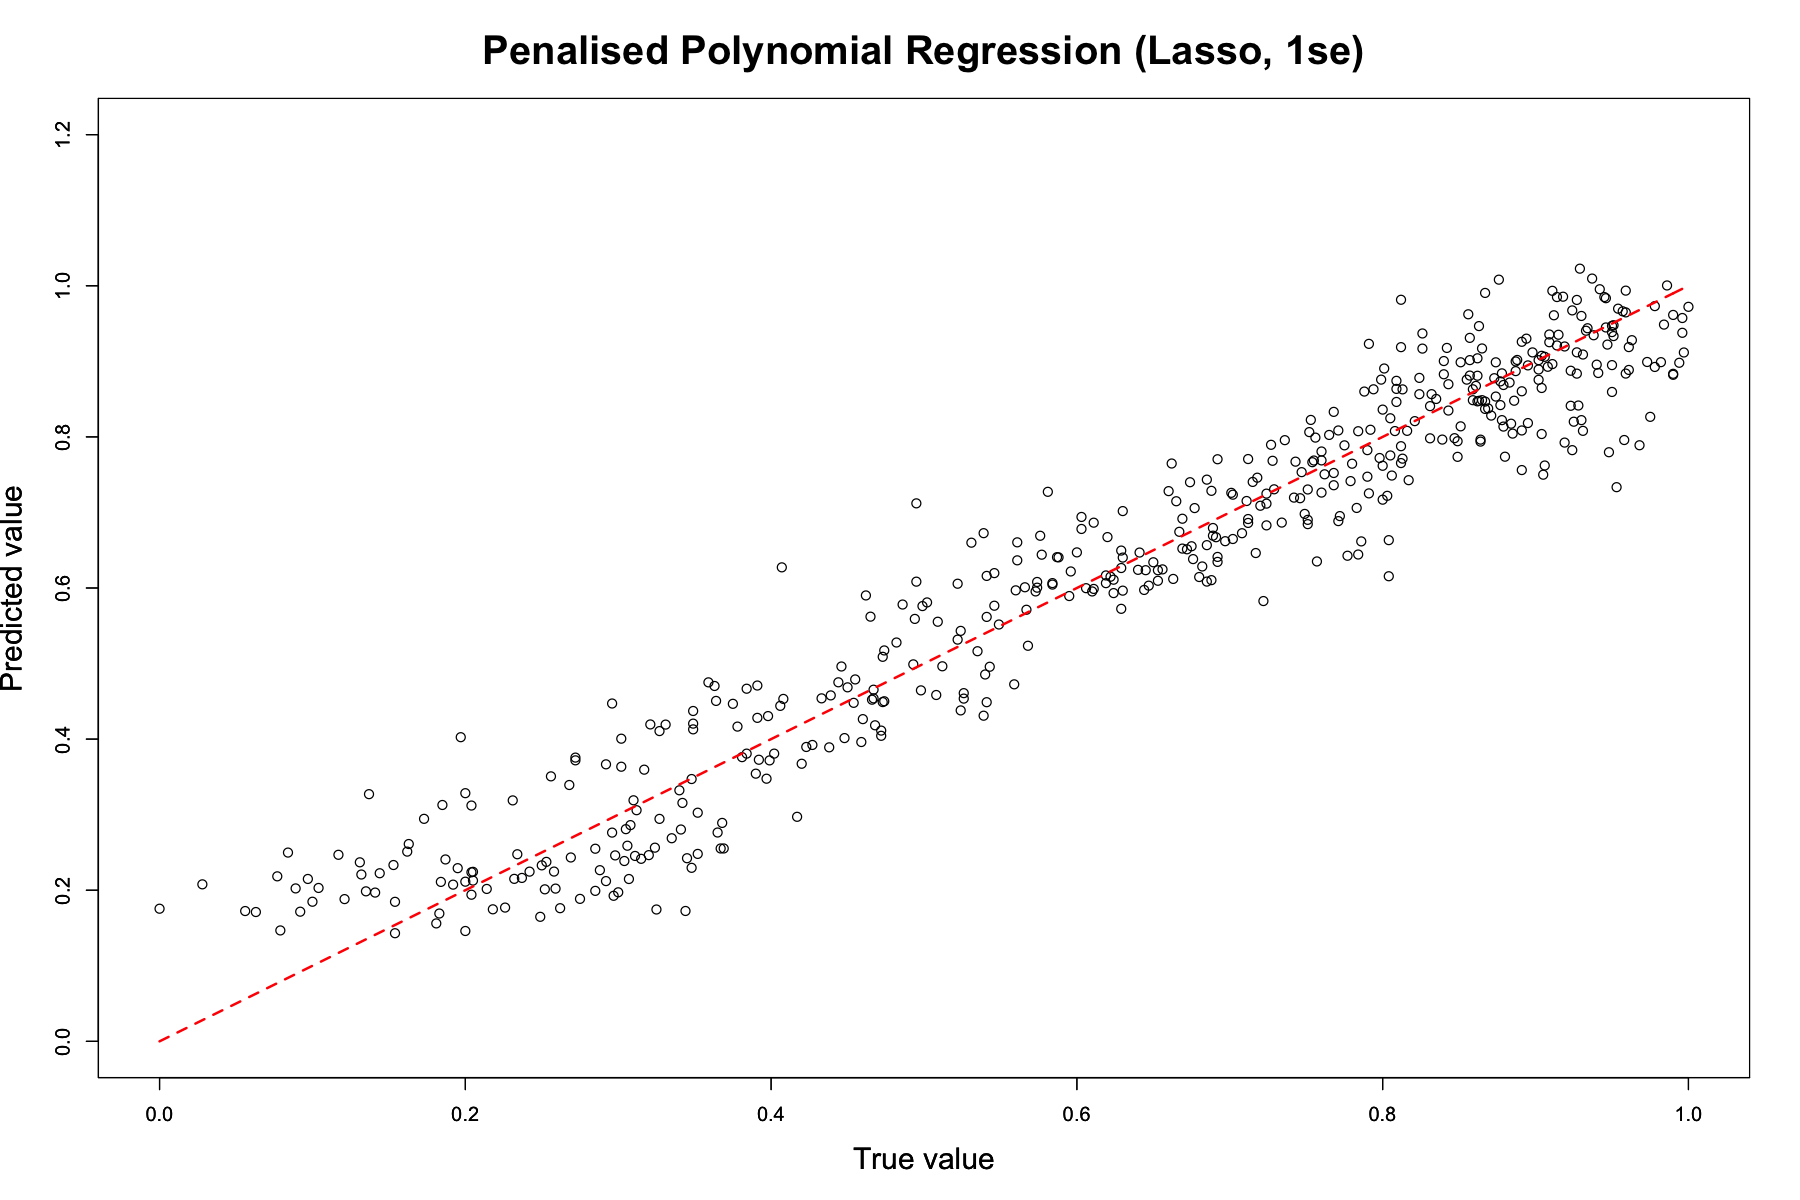
\includegraphics[width = 1.0\textwidth]{Figure/4.2.5-PPR-1se.png}
\caption{The predicted Arctic sea ice extent value vs the real Arctic sea ice extent value with Penalised Polynomial Regression (Lasso, 1se). The red referenced dotted line represents the straight line y=x. Mean Square Error (MSE) is 0.00484.}
\label{4.2.5-PPR-1se}
\end{figure}



\subsection{Random Forest} %4.2.6

\begin{figure}[htbp]
\centering
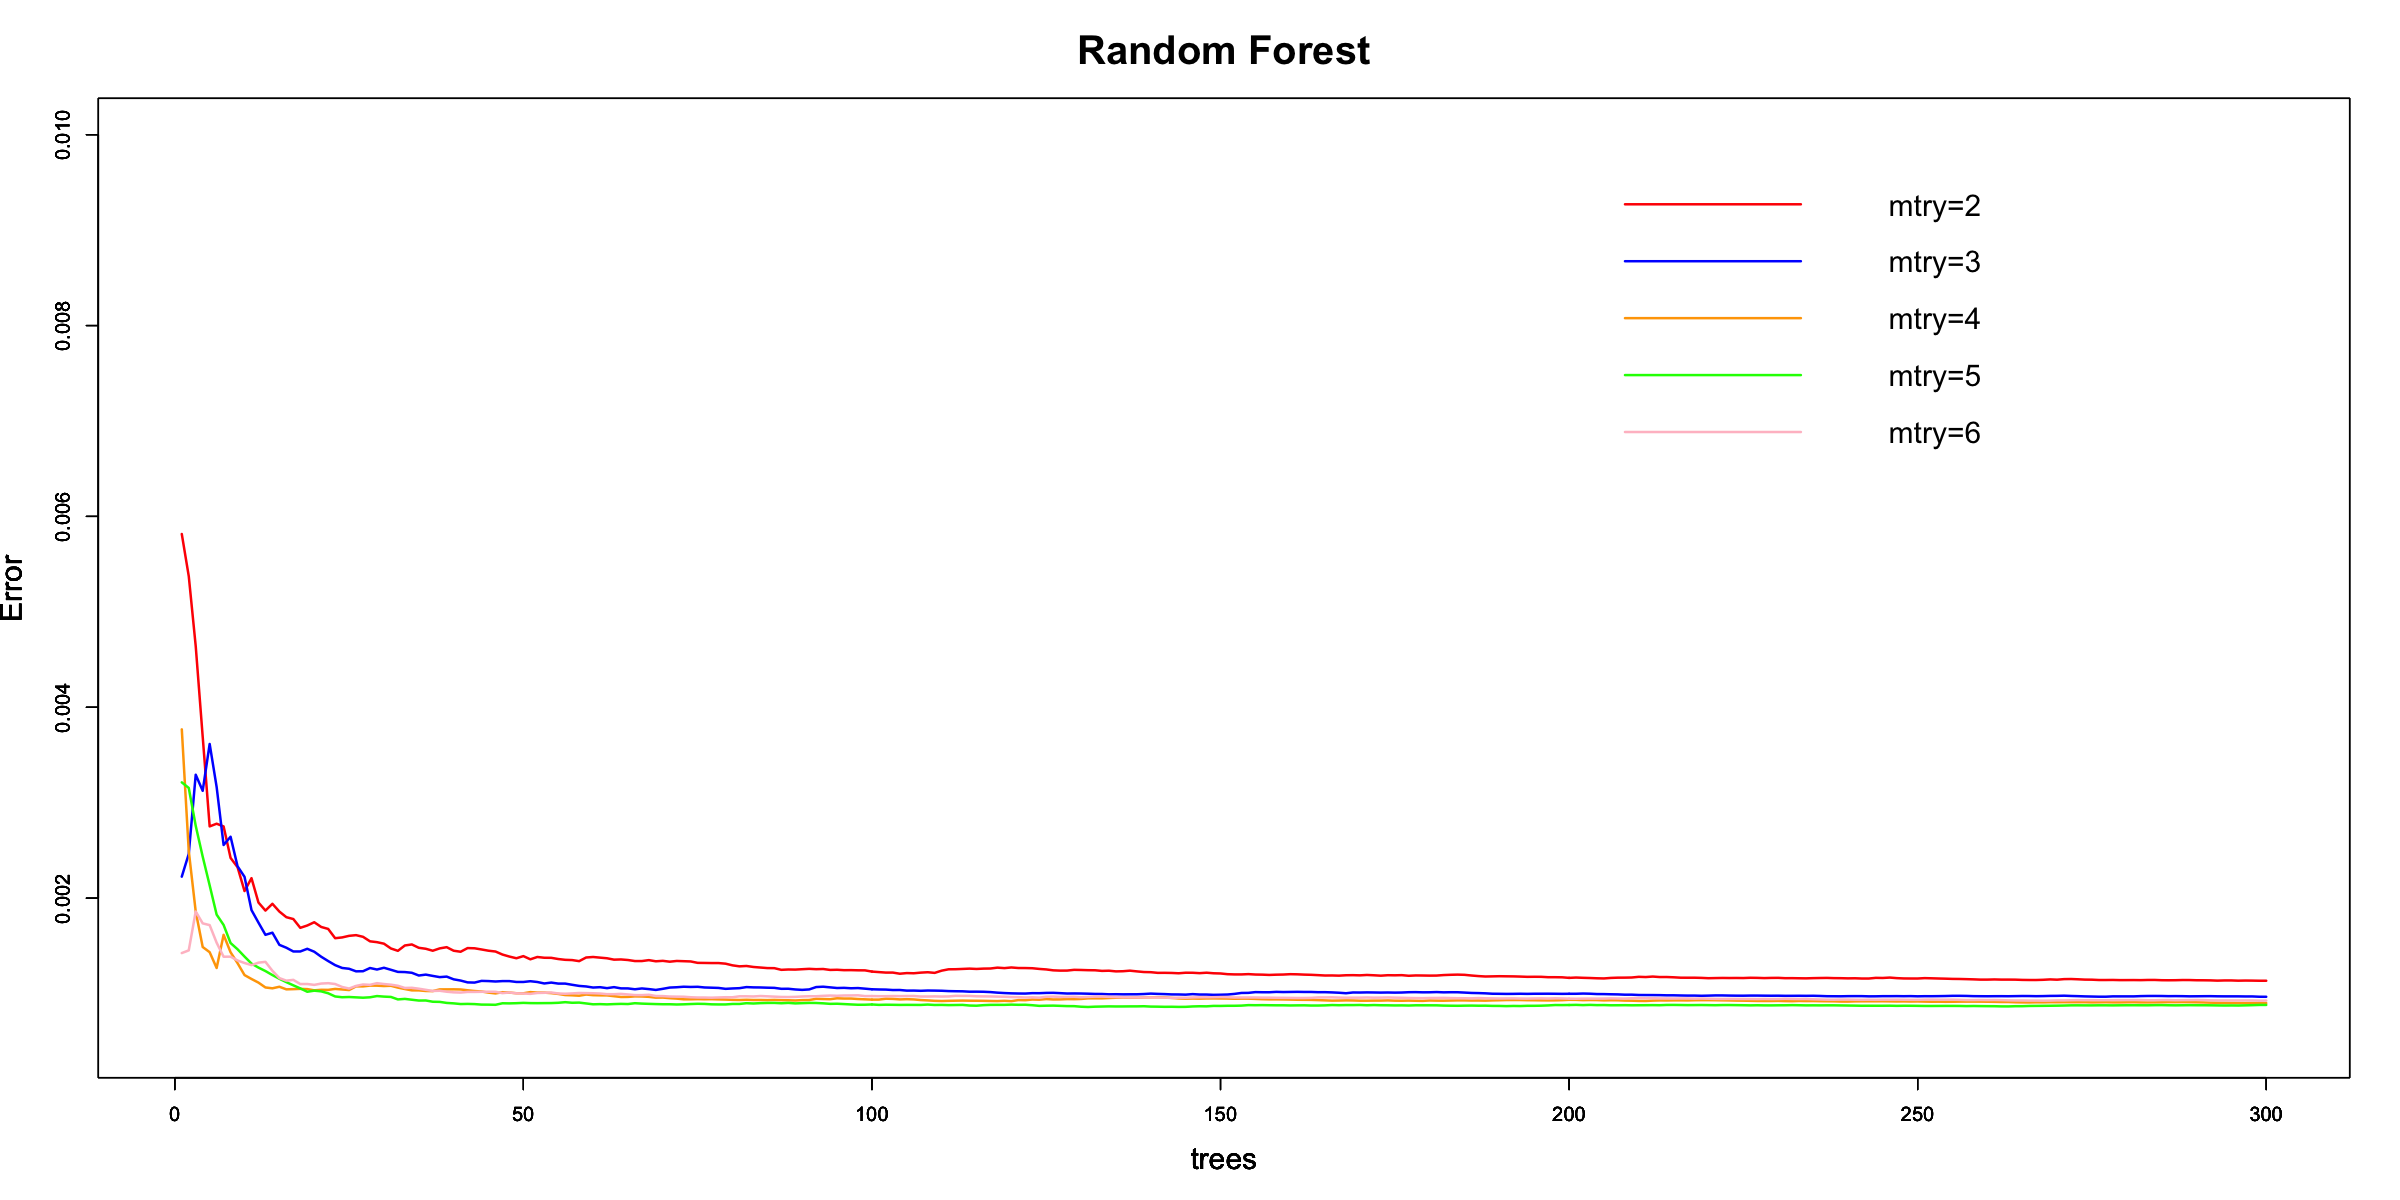
\includegraphics[width = 1.0\textwidth]{Figure/4.2.6-RF-200TreesStable.png}
\caption{Check the error stability of random forest with different number of trees.}
\label{4.2.6-RF-200TreesStable}
\end{figure}

\begin{figure}[htbp]
\centering
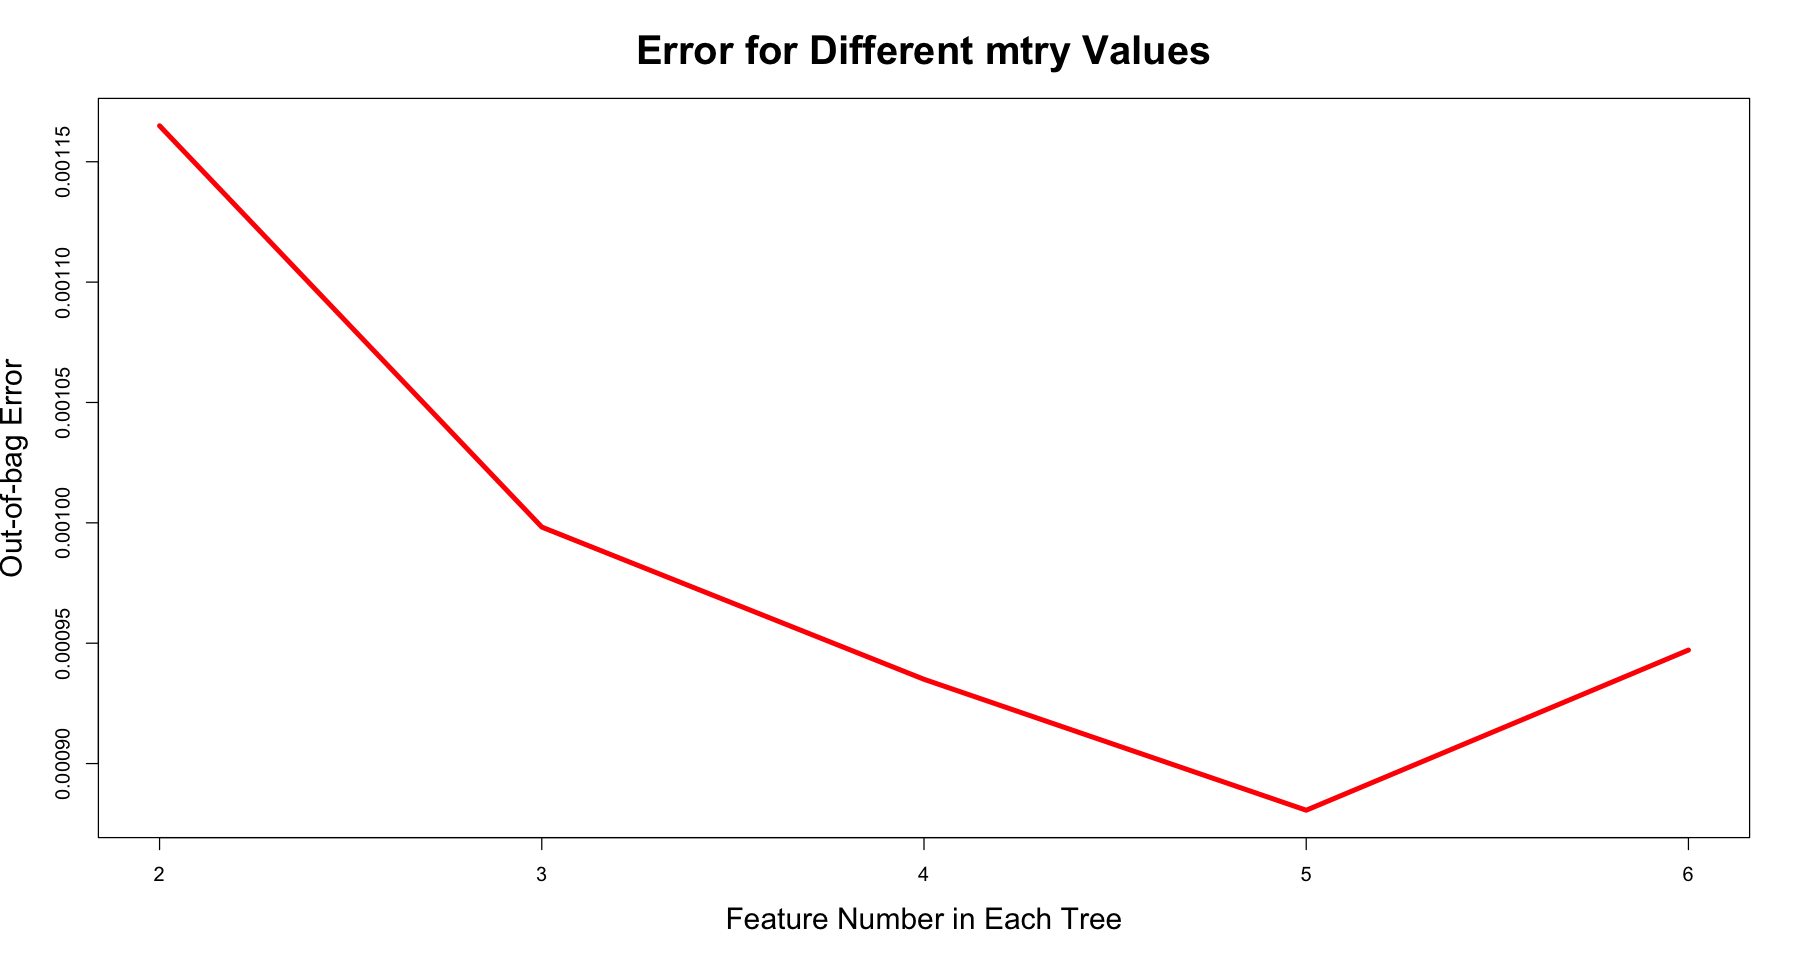
\includegraphics[width = 1.0\textwidth]{Figure/4.2.6-RF-5Features.png}
\caption{Check the out-of-bag error of random forest with different number of features in each tree when three number is 200.}
\label{4.2.6-RF-5Features}
\end{figure}

\begin{figure}[htbp]
\centering
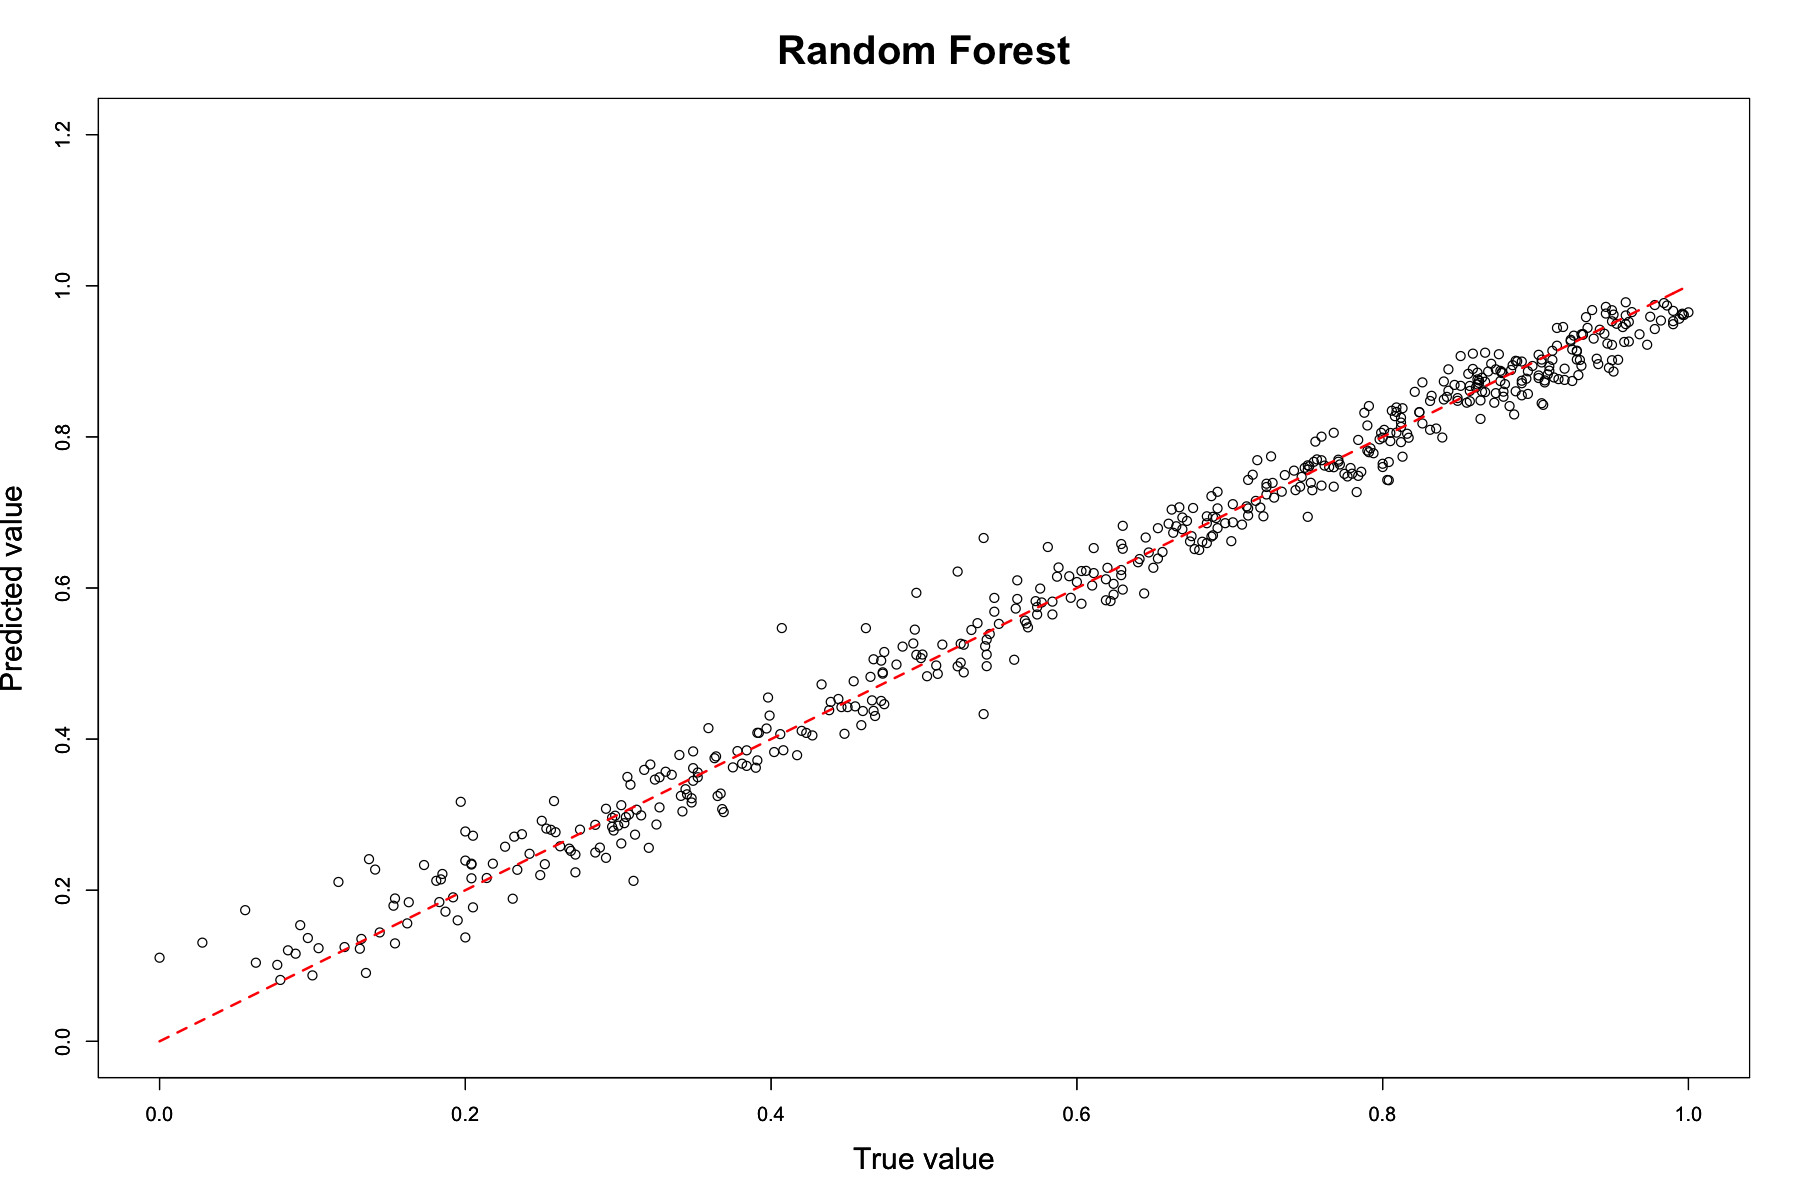
\includegraphics[width = 1.0\textwidth]{Figure/4.2.6-RF.png}
\caption{The predicted Arctic sea ice extent value vs the real Arctic sea ice extent value with Random Forest (200 trees, 5 features). The red referenced dotted line represents the straight line y=x. Mean Square Error (MSE) is 0.00105.}
\label{4.2.6-RF}
\end{figure}



\subsection{Neural Network} %4.2.7

\begin{figure}[htbp]
\centering
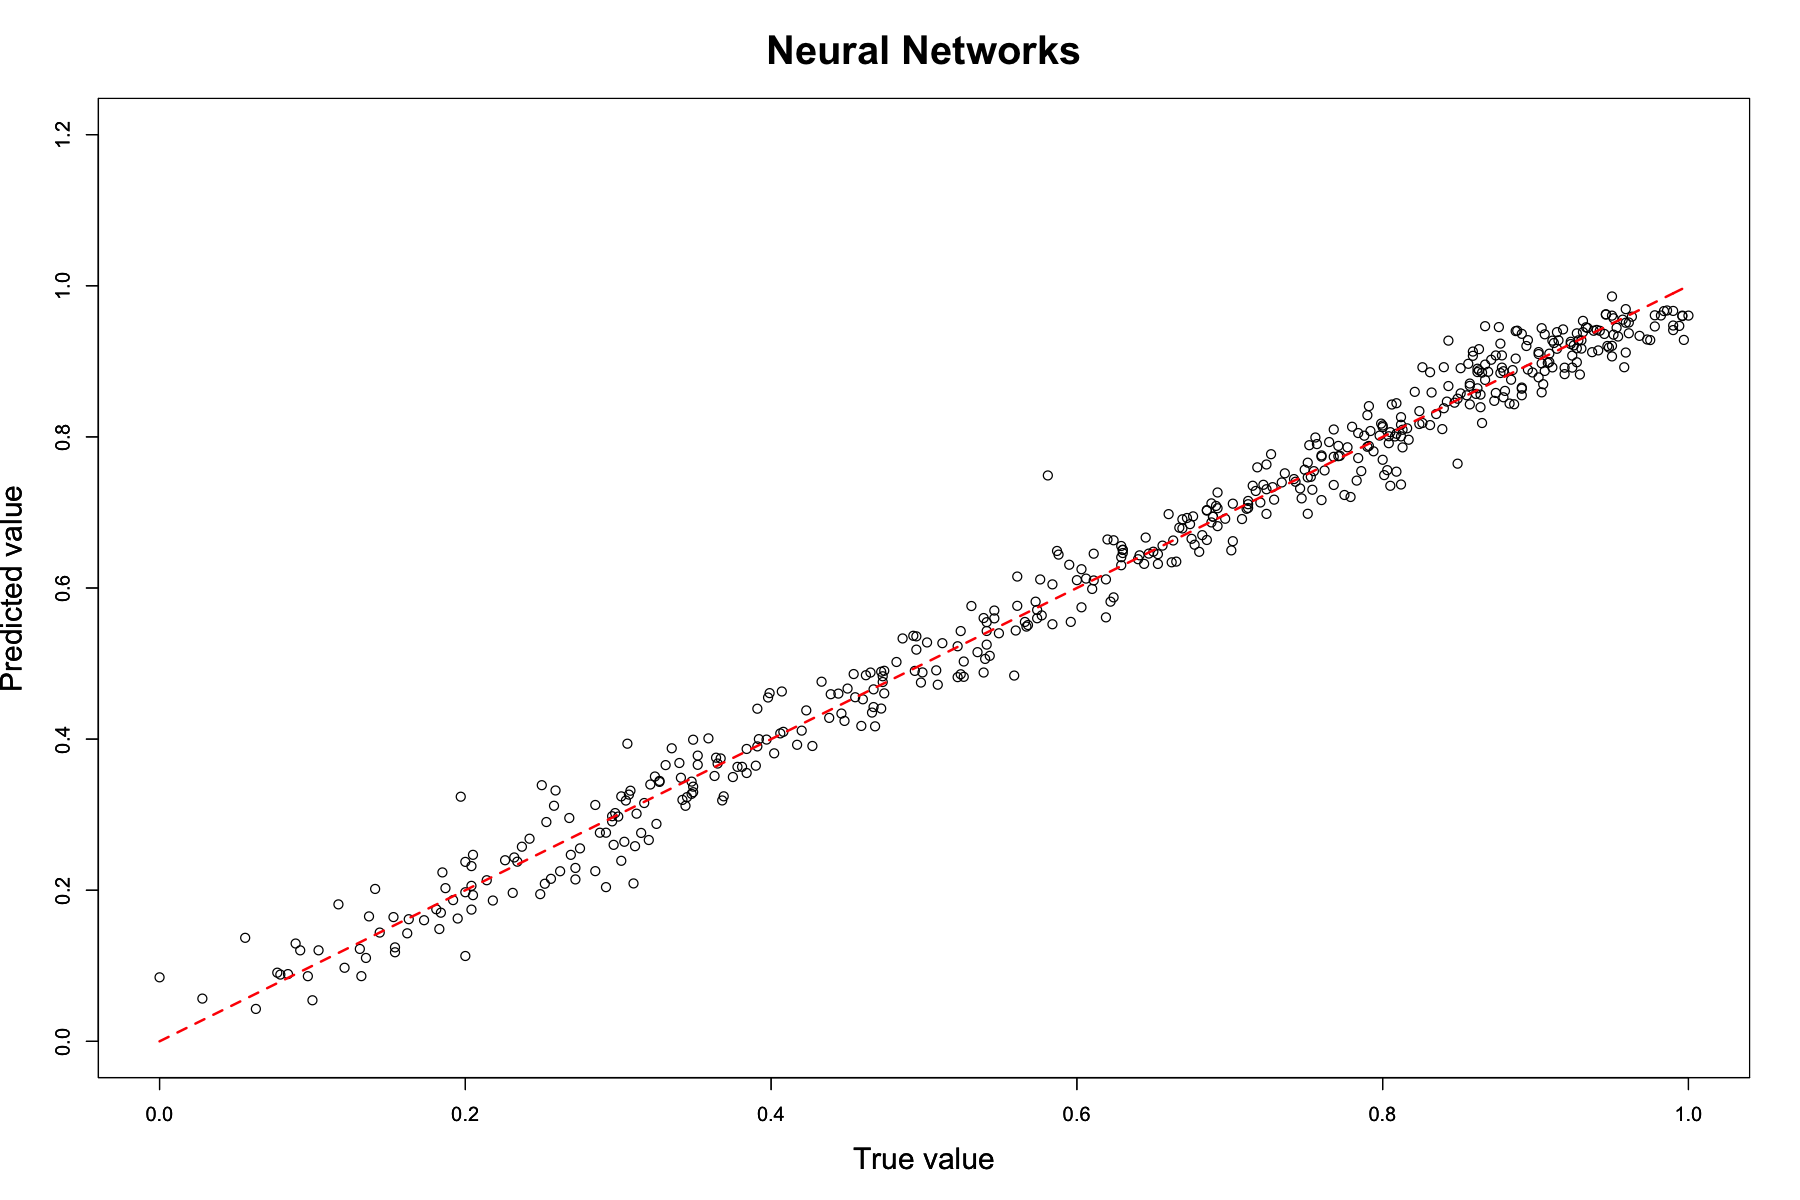
\includegraphics[width = 1.0\textwidth]{Figure/4.2.7-NN.png}
\caption{The predicted Arctic sea ice extent value vs the real Arctic sea ice extent value with Neural Networks (9 neurons, 5 hidden layers with (9,7,5,4,3) nodes respectively). The red referenced dotted line represents the straight line y=x. Mean Square Error (MSE) is 0.00104.}
\label{4.2.7-NN}
\end{figure}



\subsection{Comparison} %4.2.8

